\documentclass{../acm_proc_article-me11_tweaked}
\usepackage[usenames,dvipsnames,svgnames,table]{xcolor}
\usepackage{graphicx}
\usepackage{url}
\usepackage{caption}
\DeclareCaptionType{copyrightbox}
\usepackage{subcaption}
\begin{document}

\conferenceinfo{\textit{MediaEval 2013 Workshop,}}{October 18-19, 2013, Barcelona, Spain}

\title{An investigation of techniques that aim to improve the quality of labels provided by the crowd}

%
\def\sharedaffiliation{%
\end{tabular}
\begin{tabular}{c}}
%

\numberofauthors{1}
\author{
	\alignauthor
	Jonathon Hare, Anna Weston, Elena Simperl\\
    \email{jsh2@ecs.soton.ac.uk, aw3g10@ecs.soton.ac.uk, E.Simperl@soton.ac.uk} \\
	Sina Samangooei, David Dupplaw, Paul Lewis\\
	\email{ss@ecs.soton.ac.uk, dpd@ecs.soton.ac.uk, phl@ecs.soton.ac.uk}\\
	\affaddr{Electronics and Computer Science, University of Southampton, United Kingdom}
	\and
	\alignauthor
	Maribel Acosta\\
	\email{maribel.acosta@kit.edu} \\
	\affaddr{Institute AIFB, Karlsruhe Institute of Technology, Germany}
}

\maketitle
\begin{abstract}
The 2013 MediaEval Crowdsourcing task looked at the problem of working with noisy crowdsourced annotations of image data. The aim of the task was to investigate possible techniques for estimating the true labels of an image by using the set of noisy crowdsourced labels, and possibly any content and metadata from the image itself. For the runs in this paper, we've applied a shotgun approach and tried a number of existing techniques, which include generative probabilistic models and further crowdsourcing.
\end{abstract}

\section{Introduction}
Crowdsourcing is increasingly becoming a popular way of extracting information. One problem with crowdsourcing is that the workers can have a number of traits that affect the quality of the work they are performing. One standard way of dealing with the problem of noisy data is to ask multiple workers to perform the same task and then combine the labels of the workers in order to obtain a final estimate.

Perhaps the most intuitive way of combining labels of multiple workers is through majority voting, however other possibilities exist. The aim of the 2013 MediaEval Crowdsourcing task~\cite{CS2013} was to explore techniques in which better estimates of the true labels can be created. Our run submissions for this task explore a number of techniques to achieve this: probabilistic models of workers (i.e. estimating which workers are bad, and discounting their votes), additional crowdsourcing of images without a clear majority vote, and joint probabilistic models that take into account both the crowdsourced votes as well as extracted features.
	
\section{Methodology}
As described previously, the overall methodology for our run submissions was to take a \emph{shotgun} approach and try three fundamentally different approaches (generative probabilistic model of workers; extra crowdsourcing; and joint modelling) to the problem. The techniques and data we used for each run are summarised in Table~\ref{tab:config}. Specific details on each run are given below.

\begin{table*}[t]
	\small
	\centering
	\caption{\label{tab:config}Configuration of the submitted runs.}
	\begin{tabular}{|l||c|c|c|c|c||c|c|c|}
		\hline	
		& \multicolumn{5}{c||}{\textbf{Data}} & \multicolumn{3}{c|}{\textbf{Technique}}\\
		\cline{2-9}
	& Provided & \multicolumn{2}{c|}{Additional Labels} & \multicolumn{2}{c||}{Features} & Majority & Probabilistic & Probabilistic\\
	\cline{3-6}
	Run \# & Labels & \emph{Crowdsourced} & \emph{Expert} & \emph{Metadata} & \emph{Visual} & vote & Worker & Joint\\
	
	\hline\hline
	1 & \checkmark & & & & & & \checkmark & \\ \hline
	2 & \checkmark & \checkmark & \checkmark & & & \checkmark & & \\ \hline
	3 & \checkmark & \checkmark & \checkmark & & & & \checkmark & \\ \hline
	4 & \checkmark & \checkmark & \checkmark & \checkmark & & & & \checkmark \\ \hline
	5 & \checkmark & \checkmark & \checkmark & \checkmark & \checkmark & & &\checkmark \\ \hline
	\end{tabular}
\end{table*}

%\newpage
\subsection{Run 1}
The first run was required to only make use of the provided crowdsourced labels. For this run, we applied the generative model developed by Paul Mineiro~\cite{Mineiro20110124} illustrated in Figure~\ref{fig:model1}. This model extends the one by Whitehill et al.~\cite{NIPS2009_0100} by incorporating a hierarchical Gaussian prior on the elements of the confusion matrix (i.e. the $\gamma$ hyper-parameter in the figure). Briefly, the model assumes an unobserved ground truth label $z$ combines with a per-worker model parametrized by vector $\alpha$ and scalar item difficulty $\beta$ to generate an observed worker label $l$ for an image. The hyper-parameter $\gamma$ moderates the worker reliability as a function of the label class. The model parameters are learnt using a `Bayesian' Expectation-Maximisation algorithm. For our experiments with this model, we used the \texttt{nominallabelextract} implementation published by Paul Mineiro\footnote{\url{http://code.google.com/p/nincompoop/downloads/}} with uniform class priors. Note that the software was applied to data from each of the two questions asked of the workers separately, and ``NotSure'' answers were treated as unknowns (not included in the input data).

\begin{figure}[t]
\centering
\begin{subfigure}[t]{0.48\columnwidth}
	\centering
	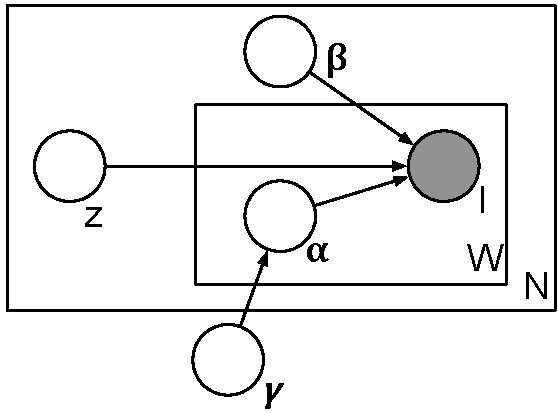
\includegraphics[width=0.7\columnwidth]{images/model1}
	\caption{\label{fig:model1}}
\end{subfigure}
\begin{subfigure}[t]{0.48\columnwidth}
	\centering
	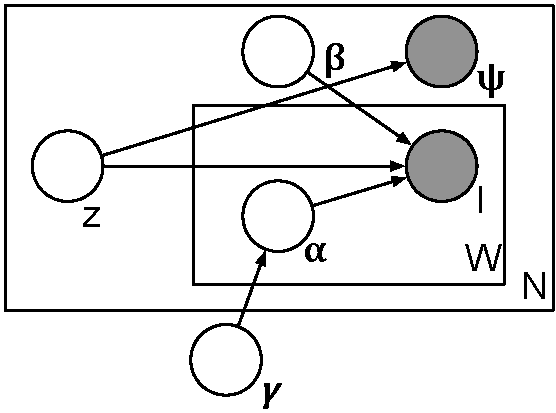
\includegraphics[width=0.7\columnwidth]{images/model2}
	\caption{\label{fig:model2}}
\end{subfigure}
\caption{Generative model of crowdworkers: (a) incorporating per-item difficulty and per-worker reliability; (b) incorporating per-item difficulty, per-worker reliability and features describing the image.}
\end{figure}
	
\subsection{Run 2}
For the second run, we gathered additional data in two ways. Firstly, we randomly selected 1000 images from the test set and had them annotated by two reliable \emph{experts}. The two experts firstly annotated the data independently and came to agreement on 671 of these (across both questions). For the images they didn't agree on for either question, they collaboratively came to a decision about the true label for both questions. The relatively low-level of initial agreement between the experts is an indication of the subjectiveness of the labelling task being performed (especially with respect to question 1 ``is this a fashion image''). Secondly, for the images in the test set that had at least two ``NotSure'' answers, we gathered more responses through additional crowdsourcing using the CrowdFlower\footnote{\url{http://crowdflower.com}} platform. In total we gathered additional an 824 responses over 421 images from this extra crowdsourcing. In order to produce the estimates we performed majority voting. 

\subsection{Run 3}
In the third run, we applied the model used in run 1 to the data in run 2. The original worker labels and additional crowdsourced labels were combined and used as the primary input. The expert labels were used to \emph{clamp} the model at the respective images in order to obtain a better fit.

\subsection{Run 4}
In the fourth run, we chose to explore the use of another generative model developed by Paul Mineiro~\cite{Mineiro20111116}. This model is inspired by the work of Raykar et al.~\cite{Raykar:2010:LC:1756006.1859894}, and incorporates the notion of the hidden unknown true label also generating a set of observed features ($\psi$). This is illustrated in the plate diagram shown in Figure~\ref{fig:model2}.

Mineiro developed an online procedure to learn the model parameters that jointly learns a logistic regressor to learn how to create classifications (estimations of the true label) from the features. A nice feature of this approach is that in each iteration of learning/fitting, the worker model informs the classifier and the classifier informs the worker model.

For this run, the features used were bag-of-words features extracted from the tags, titles, descriptions, contexts and notes metadata of each image.

\subsection{Run 5}
Finally, for the fifth run, we applied the same technique as used in run 4, but also incorporated a Pyramid Histogram of Words (PHOW) feature extracted from the images themselves on top of the metadata features. The PHOW features were created from dense SIFT features quantised into 300 visual words and aggregated into a pyramid with $2{\times}2$ and $4{\times}4$ blocks.

\section{Results and Discussion}
The results of the five runs are shown in Table~\ref{tab:results}. Whilst we can't currently make global comments as to how well these runs performed compared to na\"ive majority voting, we can note a few points. Firstly, looking at runs 2 and 3 which used the same data, we can see that the generative model used in run 3 had a minor improvement for the second label, but it had a big negative effect for the first label. It's also clear that the more advanced model (runs 4 \& 5), that took into account features, also performed less well with this data than hoped. Interestingly, when we applied both generative models to the smaller MMSys dataset we had a slight improvement. One possible reason for the relatively low performance of the generative models on the first label could well be due to the subjectiveness of the question being asked, which would lead to errors when fitting the models. This would also help indicate why additional crowdsourcing seems to improve results.

\begin{table}
	\small
	\centering
	\caption{\label{tab:results}Results for each run and label.}
	\begin{tabular}{|c|c|c|}
		\hline
		Run \# & Label 1 F1 Score & Label 2 F1 Score \\ \hline \hline
		1 & 0.7352 & 0.7636 \\ \hline
		2 & 0.8377 & 0.7621 \\ \hline
		3 & 0.7198 & 0.7710 \\ \hline
		4 & 0.7097 & 0.7528 \\ \hline
		5 & 0.6427 & 0.6026 \\ \hline
	\end{tabular}
\end{table}

\section{Acknowledgments}
The described work was funded by the Engineering and Physical Sciences Research Council under the SOCIAM platform grant, and European Union Seventh Framework Programme (FP7/2007-2013) under grant agreements 270239 (ARCOMEM) and 287863 (TrendMiner).

\bibliographystyle{abbrv}
\bibliography{../bibliography}
\end{document}
